\documentclass[11pt]{article} 
\usepackage[english]{babel}
\usepackage[utf8]{inputenc}
\usepackage[margin=0.5in]{geometry}
\usepackage{amsmath}
\usepackage{amsthm}
\usepackage{amsfonts}
\usepackage{amssymb}
\usepackage[usenames,dvipsnames]{xcolor}
\usepackage{graphicx}
\usepackage[siunitx]{circuitikz}
\usepackage{tikz}
\usepackage[colorinlistoftodos, color=orange!50]{todonotes}
\usepackage{hyperref}
\usepackage[numbers, square]{natbib}
\usepackage{fancybox}
\usepackage{epsfig}
\usepackage{soul}
\usepackage[framemethod=tikz]{mdframed}
\usetikzlibrary{positioning, automata, backgrounds}
\usepackage[shortlabels]{enumitem}
\usepackage[version=4]{mhchem}
\usepackage{multicol}
\usepackage{forest}
\usepackage{mathtools}
\usepackage{comment}
\usepackage{enumitem}
\usepackage[utf8]{inputenc}
\usepackage[linesnumbered,ruled,vlined]{algorithm2e}
\usepackage{listings}
\usepackage{color}
\usepackage[numbers]{natbib}
\usepackage{subfiles}
\usepackage{tkz-berge}


\newtheorem{prop}{Proposition}[section]
\newtheorem{thm}{Theorem}[section]
\newtheorem{lemma}{Lemma}[section]
\newtheorem{cor}{Corollary}[prop]

\theoremstyle{definition}
\newtheorem{definition}{Definition}

\theoremstyle{definition}
\newtheorem{required}{Problem}

\theoremstyle{definition}
\newtheorem{ex}{Example}


\newcommand{\interval}[4]{\draw (#2, #1) -- (#3, #1); % Usage: \interval{height}{start}{end}{label}
\draw (#2, #1-0.11) -- (#2, #1+0.11); % draw left whisker
\draw (#3, #1-0.11) -- (#3, #1+0.11); % draw right whisker
\node[] at (#2-0.25, #1) {#4};
}

\setlength{\marginparwidth}{3.4cm}
%#########################################################

%To use symbols for footnotes
\renewcommand*{\thefootnote}{\fnsymbol{footnote}}
%To change footnotes back to numbers uncomment the following line
%\renewcommand*{\thefootnote}{\arabic{footnote}}

% Enable this command to adjust line spacing for inline math equations.
% \everymath{\displaystyle}

% _______ _____ _______ _      ______ 
%|__   __|_   _|__   __| |    |  ____|
%   | |    | |    | |  | |    | |__   
%   | |    | |    | |  | |    |  __|  
%   | |   _| |_   | |  | |____| |____ 
%   |_|  |_____|  |_|  |______|______|
%%%%%%%%%%%%%%%%%%%%%%%%%%%%%%%%%%%%%%%

\title{
\normalfont \normalsize 
\textsc{CSCI 3104 Spring 2022 \\ 
Instructor: Profs. Chen and Layer} \\
[10pt] 
\rule{\linewidth}{0.5pt} \\[6pt] 
\huge Problem Set 3 \\
\rule{\linewidth}{2pt}  \\[10pt]
}
%\author{Your Name}
\date{}

\begin{document}
\definecolor {processblue}{cmyk}{0.96,0,0,0}
\definecolor{processred}{rgb}{200, 0, 0}
\definecolor{processgreen}{rgb}{0, 255, 0}
\DeclareGraphicsExtensions{.png}
\DeclareGraphicsExtensions{.gif}
\DeclareGraphicsExtensions{.jpg}

\maketitle


%%%%%%%%%%%%%%%%%%%%%%%%%
%%%%%%%%%%%%%%%%%%%%%%%%%%
%%%%%%%%%%FILL IN YOUR NAME%%%%%%%
%%%%%%%%%%AND STUDENT ID%%%%%%%%
%%%%%%%%%%%%%%%%%%%%%%%%%%
\noindent
Due Date \dotfill \textbf{February 8, 2022} \\
Name \dotfill \textbf{Julia Troni} \\
Student ID \dotfill \textbf{109280095} \\
Collaborators \dotfill \textbf{Null}

\tableofcontents

\section{Instructions}
 \begin{itemize}
	\item The solutions \textbf{must be typed}, using proper mathematical notation. We cannot accept hand-written solutions. \href{http://ece.uprm.edu/~caceros/latex/introduction.pdf}{Here's a short intro to \LaTeX.}
	\item You should submit your work through the \textbf{class Canvas page} only. Please submit one PDF file, compiled using this \LaTeX \ template.
	\item You may not need a full page for your solutions; pagebreaks are there to help Gradescope automatically find where each problem is. Even if you do not attempt every problem, please submit this document with no fewer pages than the blank template (or Gradescope has issues with it).

	\item You are welcome and encouraged to collaborate with your classmates, as well as consult outside resources. You must \textbf{cite your sources in this document.} \textbf{Copying from any source is an Honor Code violation. Furthermore, all submissions must be in your own words and reflect your understanding of the material.} If there is any confusion about this policy, it is your responsibility to clarify before the due date. 

	\item Posting to \textbf{any} service including, but not limited to Chegg, Reddit, StackExchange, etc., for help on an assignment is a violation of the Honor Code.

	\item You \textbf{must} virtually sign the Honor Code (see Section \ref{HonorCode}). Failure to do so will result in your assignment not being graded.
\end{itemize}


\section{Honor Code (Make Sure to Virtually Sign)} \label{HonorCode}

\begin{required}
\begin{itemize}
\item My submission is in my own words and reflects my understanding of the material.
\item Any collaborations and external sources have been clearly cited in this document.
\item I have not posted to external services including, but not limited to Chegg, Reddit, StackExchange, etc.
\item I have neither copied nor provided others solutions they can copy.
\end{itemize}

%\noindent In the specified region below, clearly indicate that you have upheld the Honor Code. Then type your name. 
\end{required}

\begin{proof}[I agree to the above, Julia Troni.]
%% Typing "I agree to the above," followed by your name is sufficient.
\end{proof}



\newpage
\section{Standard 7 - MST: safe and useless edges}

\begin{required}
Consider the weighted graph $G(V, E, w)$ below. Let $\mathcal{F} = \{ \{A, B\}, \{B, C\}, \{E, F\}\}$ be an intermediate spanning forest (indicated by the thick edges below). Label each edge that is \textbf {not} in $\mathcal{F}$ as safe, useless, or undecided. Provide a 1-2 sentence explanation for each such edge.


\begin{center}
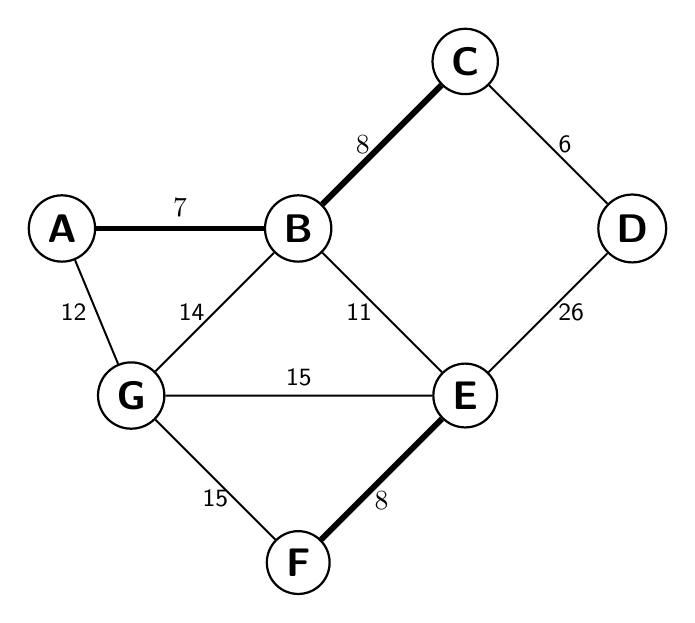
\begin{tikzpicture}[scale=0.4, auto, node distance=3cm, every loop/.style={},
  thick,main node/.style={circle,draw,font=\sffamily\Large\bfseries}]

\node[main node] (A) {A};
\node[main node] (B) [right of=A] {B};
\node[main node] (C) [above right of=B] {C};
\node[main node] (D) [below right of=C] {D};
\node[main node] (E) [below left of=D] {E};
\node[main node] (F) [below left of=E] {F};
\node[main node] (G) [above left of=F] {G};

\path[line width=0.25mm, every node/.style={font=\sffamily\small}]

(A) edge node [left]  {12} (G)
(B) edge node [left]  {11}  (E)
(C) edge node [right] {6}  (D)
(D) edge node [right] {26} (E)
(F) edge node [below] {15} (G)
(G) edge node [left]  {14} (B)
(G) edge node [above] {15}  (E)
;

\draw[line width=0.75mm] (A) -- node [above] {7} (B);
\draw[line width=0.75mm] (E) -- node [below] {8} (F);
\draw[line width=0.75mm] (B) -- node [left] {8} (C);
\end{tikzpicture}
\end{center}
\end{required}

\begin{proof}[Answer]
%Your answer goes here
$\{C,D\}$, $\{B,E\}$, and $\{A,G\}$ are \textbf{safe} edges with respect to  $\mathcal{F}$ because they are each the minimum weight edges that crosses a partition of the vertices (a cut), so they are each light edges. Since any light edge that connects two components in an intermediate spanning forest is safe, they are safe.  \\
$\{B,G\}$, $\{G,E\}$, $\{G,F\}$, $\{D,E\}$ are  \textbf{undecided} edges with respect to  $\mathcal{F}$ because they are neither safe, nor useless \\
There are no edges that will create a cycle with respect to $\mathcal{F}$ so there are no useless edges. \\
\begin{enumerate}
\item $\{C,D\}$ is the minimum weight edge with exactly one endpoint in the the component $\{A,B,C,G\}$ and the minimum weight edge with exactly one edge in the component $\{F,E,D\}$. Therefore $\{C,D\}$ is a light edge and hence a \textbf{safe} edge with respect to  $\mathcal{F}$
\item $\{B,E\}$ is the minimum weight edge with exactly one endpoint in the the component $\{A,B,C,G\}$ and the minimum weight edge with exactly one edge in the component $\{F,E\}$. Therefore $\{B,E\}$ is a light edge and hence a \textbf{safe} edge with respect to  $\mathcal{F}$
\item $\{A,G\}$ is the minimum weight edge with exactly one endpoint in the the component $\{A,B,C,D,E,F\}$ and the minimum weight edge with exactly one edge in the component $\{G\}$. Therefore $\{A,G\}$ is a light edge and hence a \textbf{safe} edge with respect to  $\mathcal{F}$ \\

See below for a visual of the safe edges \\

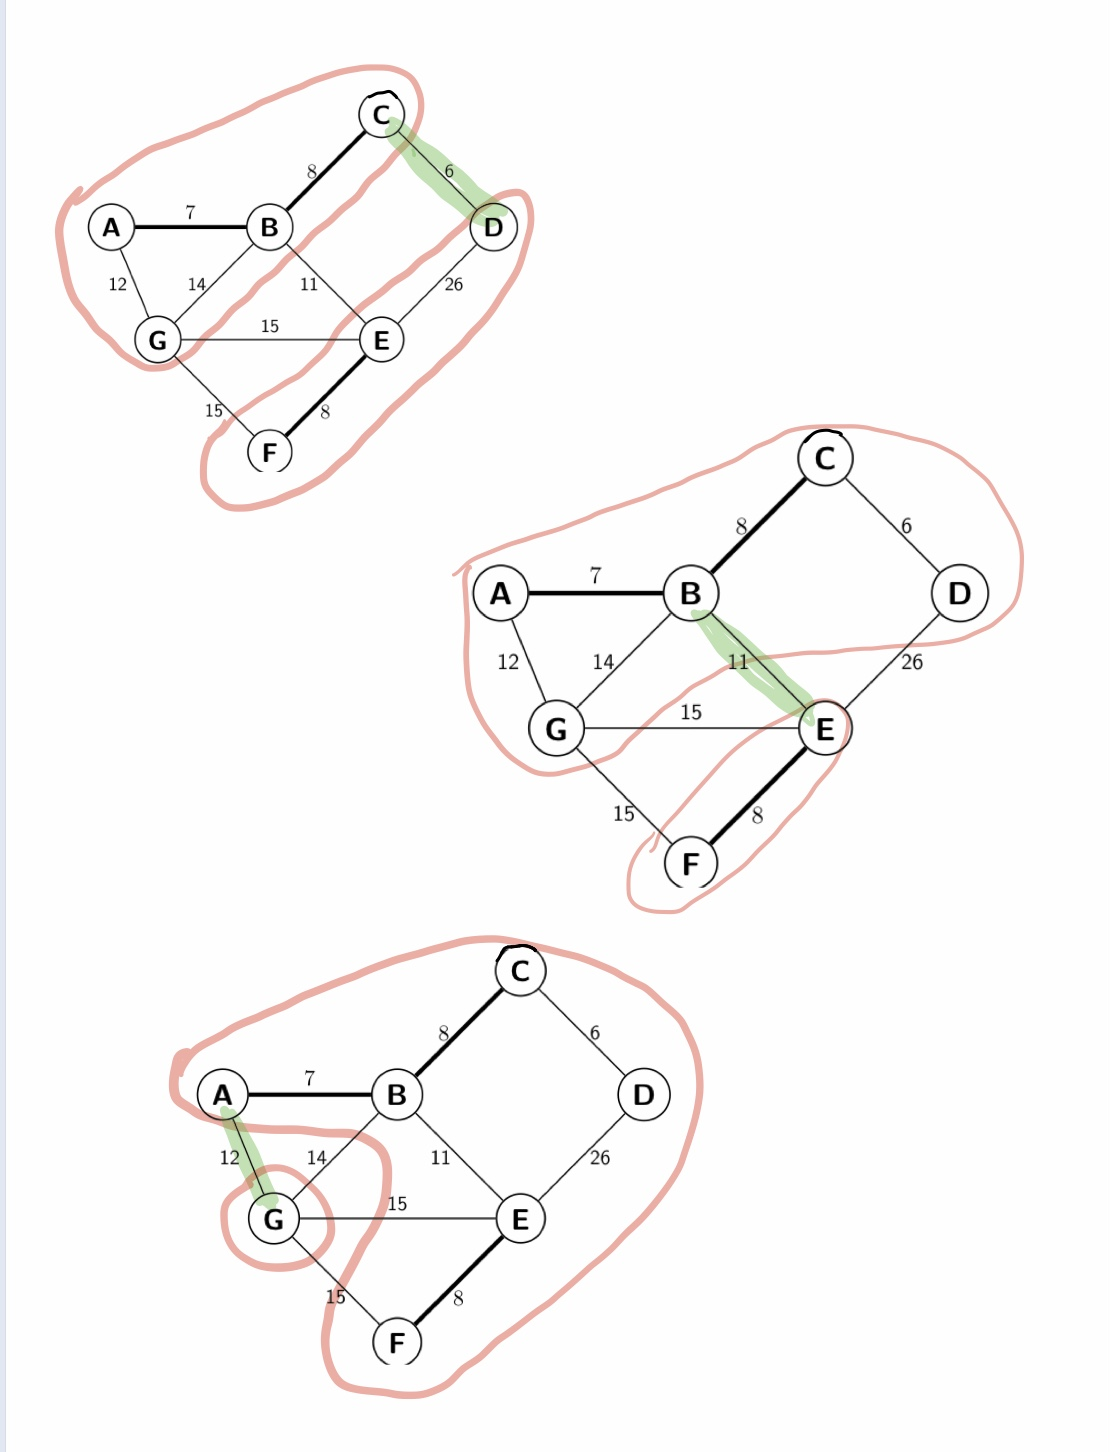
\includegraphics[width=0.7\textwidth]{hw3problem1} \\

\item While the edge $\{B,G\}$ has exactly one endpoint in the component $\{A,B,C,D,E,F\}$ and one endpoint in the component $\{G\}$, it is not a minimum weight edge in doing so. Therefore, $\{B,G\}$ is an \textbf{undecided} edge with respect to  $\mathcal{F}$
\item Similarly the edge $\{G,E\}$ has exactly one endpoint in the component $\{A,B,C,D,E,F\}$ and one endpoint in the component ${G}$, but it is not a minimum weight edge in doing so. Therefore, $\{G,E\}$ is an \textbf{undecided} edge with respect to  $\mathcal{F}$
\item Similarly the edge $\{G,F\}$ has exactly one endpoint in the component $\{A,B,C,D,E,F\}$ and one endpoint in the component $\{G\}$, although it is not a minimum weight edge connecting these components. Therefore, $\{G,F\}$ is an \textbf{undecided} edge with respect to  $\mathcal{F}$
\item Lastly, the edge $\{D,E\}$ has exactly one endpoint in the component $\{A,B,C,D,G\}$ and one endpoint in the component $\{E,F\}$, however it is not a minimum weight edge connecting these components. Therefore, $\{D,E\}$ is an \textbf{undecided} edge with respect to  $\mathcal{F}$



\end{enumerate}
\end{proof}

 
\newpage
\section{Standard 8- Kruskal's Algorithm}

\begin{required}
Consider the weighted graph $G(V, E, w)$ below. Clearly list the order in which Kruskal's algorithm adds edges to a minimum-weight spanning tree for $G$. Additionally, clearly articulate the steps that Kruskal's algorithm takes as it selects the first \textbf{three} edges.

\begin{center}
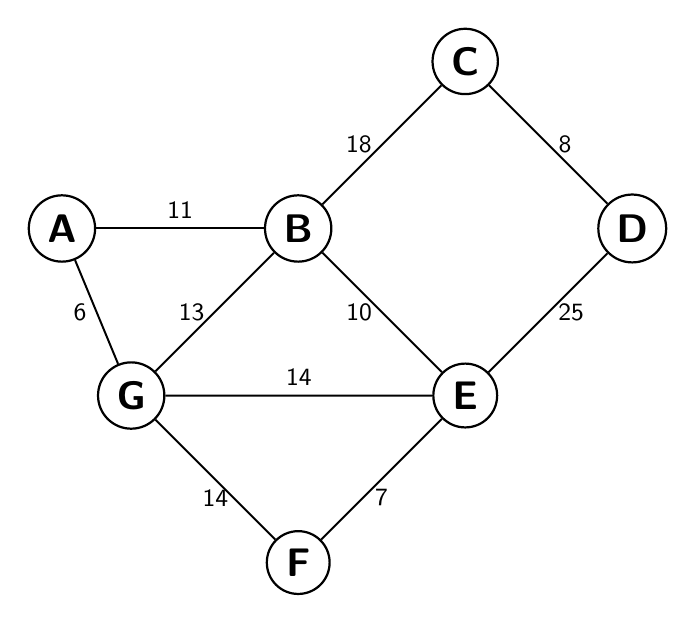
\begin{tikzpicture}[scale=0.4, auto, node distance=3cm, every loop/.style={},
  thick,main node/.style={circle,draw,font=\sffamily\Large\bfseries}]

\node[main node] (A) {A};
\node[main node] (B) [right of=A] {B};
\node[main node] (C) [above right of=B] {C};
\node[main node] (D) [below right of=C] {D};
\node[main node] (E) [below left of=D] {E};
\node[main node] (F) [below left of=E] {F};
\node[main node] (G) [above left of=F] {G};

\path[line width=0.25mm, every node/.style={font=\sffamily\small}]
(B) edge node [left]  {18} (C)
(B) edge node [left]  {10}  (E)
(C) edge node [right] {8}  (D)
(D) edge node [right] {25} (E)
(F) edge node [below] {14} (G)
(G) edge node [left]  {13} (B)
(G) edge node [above] {14}  (E)
(A) edge node [above] {11} (B)
(E) edge node [below] {7} (F)
(A) edge node [left] {6} (G)
;
\end{tikzpicture}
\end{center}
\end{required}


\begin{proof}[Answer]
%Your answer goes here

Kruskal's algorithm begins by initializing the intermediate spanning forest $\mathcal{F}$ to contain all the vertices but no edges. Then, it creates a priority queue in which it adds all of the edges of the graph, ordered from lowest weight to highest weight. \\
For this graph, the edges will be added to the queue such that initially 
\\
$Q= [ (\{A,G\}, 6), (\{E,F\}, 7), (\{C,D\}, 8), (\{B,E\}, 10), $
\\
 $(\{A,B\}, 11), (\{B,G\}, 13), (\{E,G\}, 14), (\{F,G\}, 14), (\{B,C\}, 18), (\{D,E\}, 25) ]$ \\
\begin{itemize}
\item Poll from Q, which returns $(\{A,G\}, 6)$. Since A and G are on different components of $\mathcal{F}$, $\{A,G\}$ does not create a cycle so we add it to $\mathcal{F}$. Now the edges of $\mathcal{F}$ are $ [(\{A,G\}, 6)]$ and\\
 $Q= [(\{E,F\}, 7), (\{C,D\}, 8), (\{B,E\}, 10), (\{A,B\}, 11),$ \\
$ (\{B,G\}, 13), (\{E,G\}, 14), (\{F,G\}, 14), (\{B,C\}, 18), (\{D,E\}, 25) ]$ \\
\item Poll from Q, which returns $(\{E,F\}, 7)$. Since E and F are on different components of $\mathcal{F}$, adding that edge would not create a cycle so we add the edge to $\mathcal{F}$. Now the edges of $\mathcal{F}$ are $ [(\{A,G\}, 6), (\{E,F\}, 7)]$ and\\ $Q= [(\{C,D\}, 8), (\{B,E\}, 10), (\{A,B\}, 11), (\{B,G\}, 13), (\{E,G\}, 14), (\{F,G\}, 14), (\{B,C\}, 18), (\{D,E\}, 25) ]$ \\
\item Poll from Q, which returns $(\{C,D\}, 8)$. Since C and D are on different components of $\mathcal{F}$,  adding that edge would not create a cycle so, we add the edge to $\mathcal{F}$. Now the edges of $\mathcal{F}$ are $[(\{A,G\}, 6), (\{E,F\}, 7), (\{C,D\}, 8)]$ and  \\
$Q= [ (\{B,E\}, 10), (\{A,B\}, 11), (\{B,G\}, 13), (\{E,G\}, 14), (\{F,G\}, 14), (\{B,C\}, 18), (\{D,E\}, 25) ]$ \\
\end{itemize}

The algorithm will continue in this method, polling each edge from the priority queue and checking if it creates a cycle. If it does NOT create a cycle, the edge is added to $\mathcal{F}$. However, if it does create a cycle, meaning the two vertices are on the same component of $\mathcal{F}$, then the edge will NOT be added to $\mathcal{F}$. \\
So $(\{B,E\}, 10)$ will be the next added edge, followed by  $(\{A,B\}, 11)$ and lastly  $(\{B,C\}, 18)$\\

The algorithm terminates when $\mathcal{F}$ spans all vertices, and at which point $\mathcal{F}$ has $|V(G)|-1 = 7-1= 6$ edges and is the MST of the graph. \\
For this graph, the MST $\mathcal{F}$ contains the following edges and is pictured below \\
$ [(\{A,G\}, 6), (\{E,F\}, 7), (\{C,D\}, 8), (\{B,E\}, 10), (\{A,B\}, 11),  (\{B,C\}, 18)]$. \\
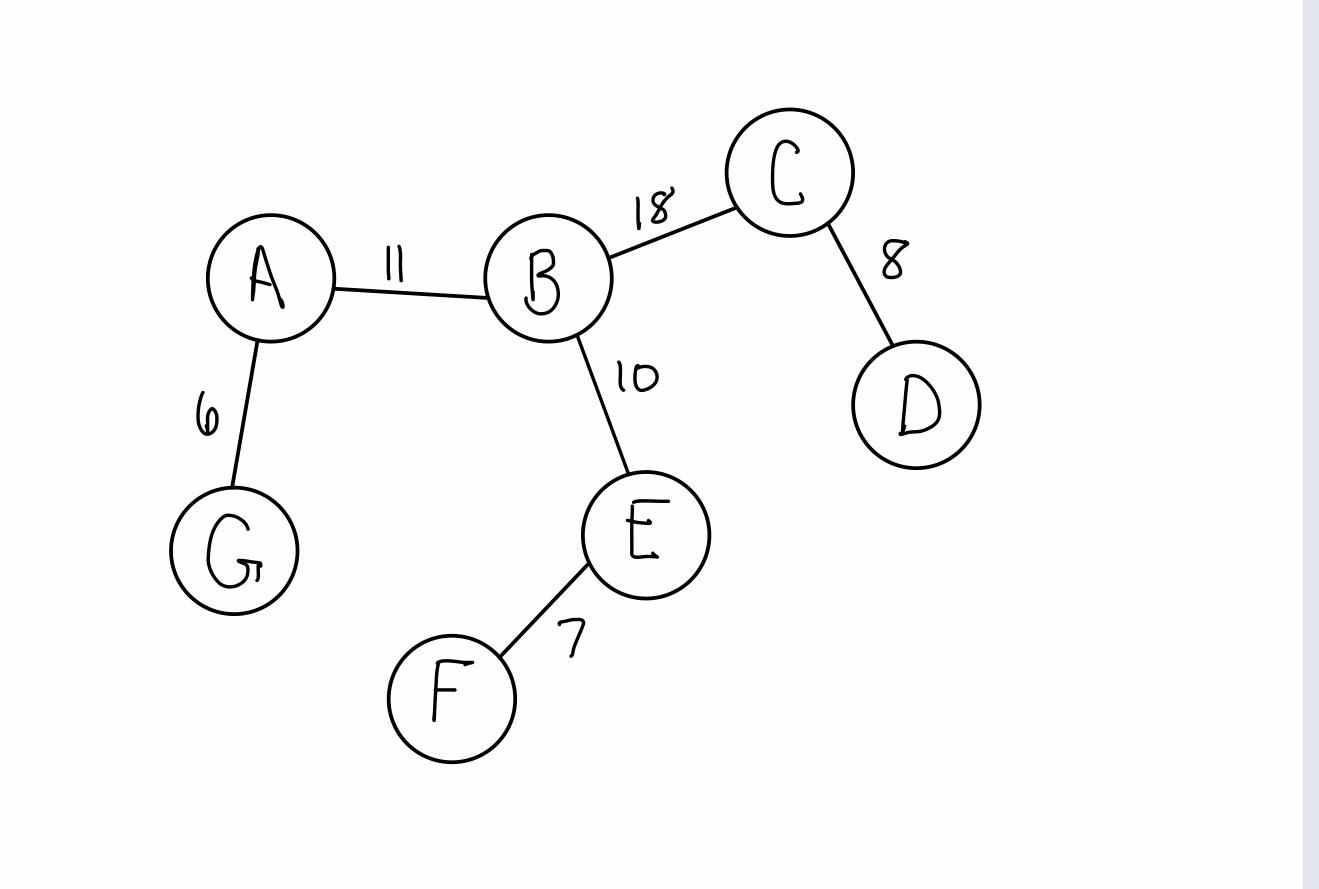
\includegraphics[width=0.7\textwidth]{hw3problem34} \\


\end{proof}


\newpage
\section{Standard 9- Prim's Algorithm}

\begin{required}
Consider the weighted graph $G(V, E, w)$ below. Clearly list the order in which Prim's algorithm, \textbf{using the source vertex} $A$, adds edges to a minimum-weight spanning tree for $G$. Additionally, clearly articulate the steps that Prim's algorithm takes as it selects the first \textbf{three} edges.

\begin{center}
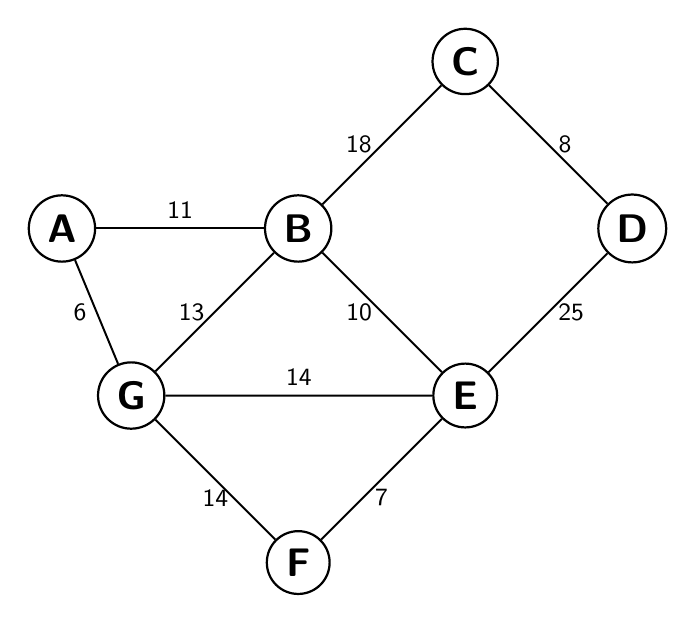
\begin{tikzpicture}[scale=0.4, auto, node distance=3cm, every loop/.style={},
  thick,main node/.style={circle,draw,font=\sffamily\Large\bfseries}]

\node[main node] (A) {A};
\node[main node] (B) [right of=A] {B};
\node[main node] (C) [above right of=B] {C};
\node[main node] (D) [below right of=C] {D};
\node[main node] (E) [below left of=D] {E};
\node[main node] (F) [below left of=E] {F};
\node[main node] (G) [above left of=F] {G};

\path[line width=0.25mm, every node/.style={font=\sffamily\small}]
(B) edge node [left]  {18} (C)
(B) edge node [left]  {10}  (E)
(C) edge node [right] {8}  (D)
(D) edge node [right] {25} (E)
(F) edge node [below] {14} (G)
(G) edge node [left]  {13} (B)
(G) edge node [above] {14}  (E)
(A) edge node [above] {11} (B)
(E) edge node [below] {7} (F)
(A) edge node [left] {6} (G)
;
\end{tikzpicture}
\end{center}
\end{required}


\begin{proof}[Answer]
%Your answer goes here 

\begin{itemize}
\item Initialize the intermediate spanning forest, $\mathcal{F}$,  to contain all of the vertices of G, but no edges. Then initialize the priority queue to contain the edges incident to the source vertex A. The priority queue will order the edges from lowest to highest weights.\\
So at the start $Q= [ (\{A,G\}, 6), (\{A,B\}, 11) ]$ 
\item Poll the edge $\{A,G\}$ from Q and mark $\{A,G\}$ as processed. $\{A,G\}$ has exactly one endpoint on the component containing A, hence it does not create a cycle, so we add $\{A,G\}$ to $\mathcal{F}$. Then push the unprocessed edges incident to G onto the queue. \\
So $Q= [ (\{A,B\}, 11), (\{G,B\}, 13), (\{G,E\}, 14), (\{G,F\}, 14) ]$ 
\item Poll the edge $\{A,B\}$ from Q and mark it as processed. $\{A,B\}$ has exactly one endpoint on the component containing A, so we add $\{A,B\}$ to $\mathcal{F}$. Then push the unprocessed edges incident to B (that are not already in Q) onto the queue. \\
So $Q= [ (\{B,E\}, 10), (\{G,B\}, 13), (\{G,E\}, 14), (\{G,F\}, 14), (\{B,C\}, 18)]$ 
\item Now poll the edge $\{B,E\}$ from Q and mark it as processed. $\{B,E\}$ has exactly one endpoint on the component containing A, so we add $\{B,E\}$ to $\mathcal{F}$. Then push the unprocessed edges incident to E (that are not already in Q) onto the queue. \\
So $Q= [ (\{E,F\}, 7), (\{G,B\}, 13), (\{G,E\}, 14), (\{G,F\}, 14), (\{B,C\}, 18), (\{E,D\}, 25)]$ 
\item Now poll the edge $\{E,F\}$ from Q and mark it as processed. $\{E,F\}$ has exactly one endpoint on the component containing A, so we add $\{E,F\}$ to $\mathcal{F}$. Since there are no edges incident to F that are not already in Q, we do not push any new edges. \\
So $Q= [ (\{G,B\}, 13), (\{G,E\}, 14), (\{G,F\}, 14), (\{B,C\}, 18), (\{E,D\}, 25)]$ 
\item Now poll the edge $\{G,B\}$ from Q and mark it as processed. As both G and B belong to the component containing A, we do NOT add it to $\mathcal{F}$.\\
Now $Q= [ (\{G,E\}, 14), (\{G,F\}, 14), (\{B,C\}, 18), (\{E,D\}, 25)]$ 
\item Now poll the edge $\{G,E\}$ from Q and mark it as processed. As both G and E belong to the component containing A, we do NOT add it to $\mathcal{F}$.\\
Now $Q= [ (\{G,F\}, 14), (\{B,C\}, 18), (\{E,D\}, 25)]$ 
\item Now poll the edge $\{G,F\}$ from Q and mark it as processed. As both G and F belong to the component containing A, we do NOT add it to $\mathcal{F}$.\\
Now $Q= [ (\{B,C\}, 18), (\{E,D\}, 25)]$ 
\item Now poll the edge $\{B,C\}$ from Q and mark it as processed. $\{B,C\}$ has exactly one endpoint on the component containing A, so we add $\{B,C\}$ to $\mathcal{F}$. Then push the unprocessed edges incident to C (that are not already in Q) onto the queue. \\
Now $Q= [ (\{C,D\}, 8), (\{E,D\}, 25)]$ 
\item Now poll the edge $\{C,D\}$ from Q and mark it as processed. $\{C,D\}$ has exactly one endpoint on the component containing A, so we add $\{C,D\}$ to $\mathcal{F}$. Since there are no edges incident to D that are not already in Q, we do not push any new edges. \\
Now $Q= [ (\{E,D\}, 25)]$ 
\item Now poll the edge $\{E,D\}$ from Q and mark it as processed. As both E and D belong to the component containing A, we do NOT add it to $\mathcal{F}$. Note: $\{E,D\}$ is the max weight edge, which will never be added to the MST \\
Now $Q= []$ and $\mathcal{F}$ has $|V(G)|-1 = 7-1= 6$ edges so the algorithm terminates and returns $\mathcal{F}$ as shown below. 
\end{itemize}
For this graph, the MST $\mathcal{F}$ contains the following edges added in this order \\
$ [(\{A,G\}, 6), (\{A,B\}, 11), (\{B,E\}, 10), (\{E,F\}, 7), (\{B,C\}, 18), (\{C,D\}, 8)]$. 

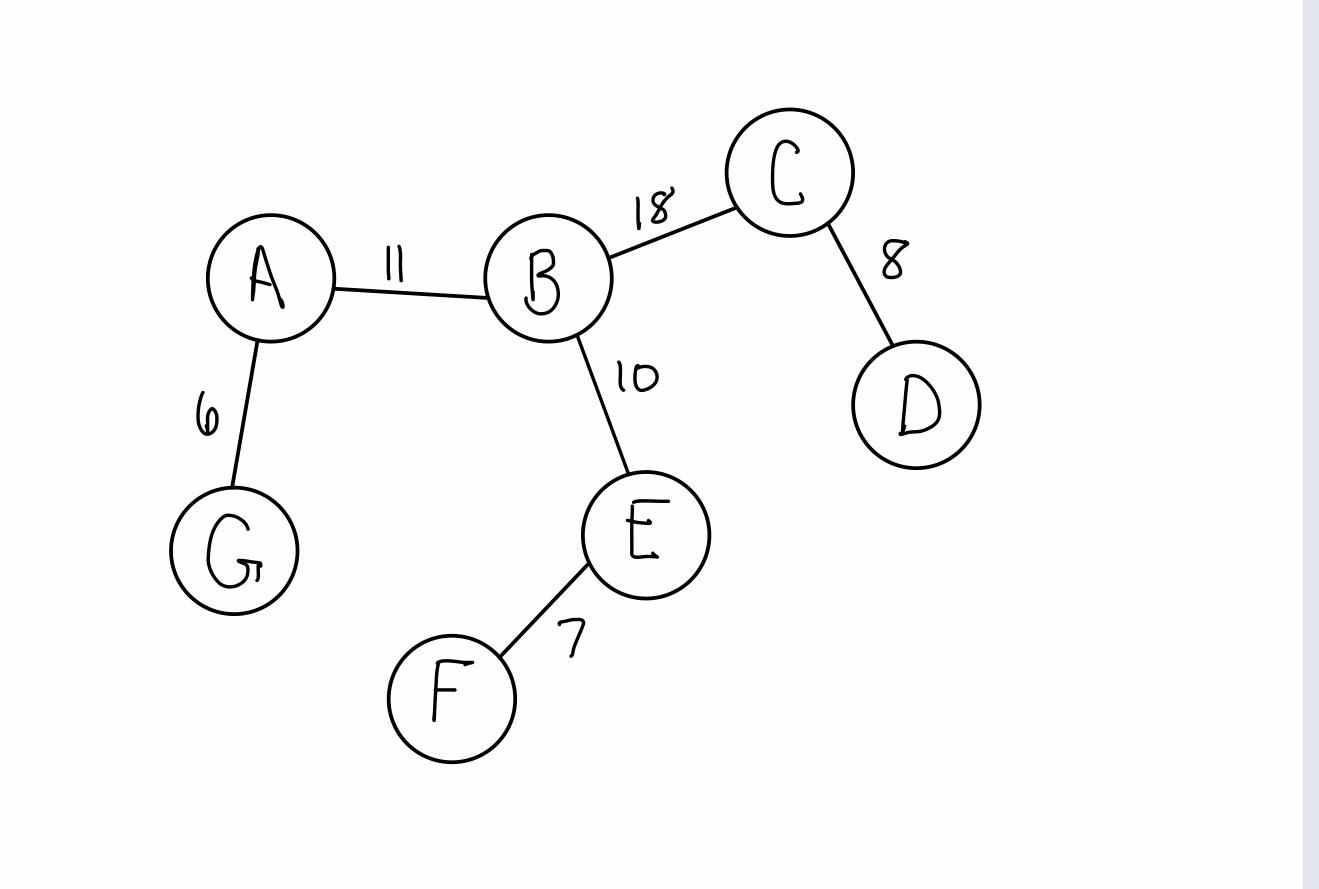
\includegraphics[width=0.7\textwidth]{hw3problem34} \\


\end{proof}
\end{document} % NOTHING AFTER THIS LINE IS PART OF THE DOCUMENT



